\documentclass[12pt]{article}

\usepackage{amsthm}
\usepackage{graphicx}

\begin{document}

\theoremstyle{definition}
\newtheorem{definition}{Definition}[section]

\theoremstyle{remark}
\newtheorem*{remark}{Remark}
\newtheorem{theorem}{Theorem}[section]
\newtheorem{lemma}[theorem]{Lemma}

\section{Maximum Matching - greedy algorithm}

\begin{theorem}
    The maximum matching greedy algorithm for interval graphs is correct.
\end{theorem}

\begin{proof}
    Let $I:= \{i_1, ... i_n\}$; with the intervals sorted by their right-end point.
    The proof is done by induction on $|I|$.\\
    For $|I|=1$, the algorithm gives $M=\emptyset$; which is correct. \\

    \textit{Induction step}\\
    Suppose the algorithm gives the correct answer for $n-1$ intervals. Let $|I| = n$, and $M$ be the matching computed by the greedy algorithm for $I-i_n$. Let $U$ be the set of unmatched intervals. \\
    If $U$ is empty, when treating $I$ the algorithm will give the same answer: $M$.\\
    Let $U$ be non empty. Let $i_k \in U$. If $i_k \cap i_n \ne \emptyset$, the algorithm will return $M+(i_k, i_n)$. 
    Indeed, for $i<k$:
    \begin{itemize}
        \item If $i_i$ could be matched with something in $I-i_n$, it would never choose to match it with $i_n$ as it is the worst choice. 
        \item If $i_i$ could not be matched in $I-i_n$, then $i_i$ will be left unmatched; because if it was possible to match it with $i_n$; then $i_i$ and $i_k$ would have not be unmatched $I-i_n$. 
    \end{itemize} 

    \textit{Augmentating path}\\
    Suppose now that $U$ is non empty, and that for some $i_k \in U$ we can find a shortest augmentating path $P: (i_k, j_1, j_1', j_2, j_2', ... , j_m', i_n)$, namely:
    \begin{itemize}
        \item $i_k \cap j_1 \ne \emptyset$ and $j_m'\cap i_n \ne \emptyset$.
        \item $\forall x<m, j_x' \cap j_{x+1} \ne \emptyset$.
        \item $(j_x$, $j_x') \in M$.
        
    \end{itemize}

    Until the end of the proof, we will use the notation $r_k, r_x, r_x'$ for the right-end points of respectively $i_k, j_x, j_x'$, and $l_k, l_x, l_x'$ for left-end points.  \\

    \textit{Decreasing property}\\
    We shall now prove by a second induction that $\forall x, r_{x+1}' < r_x'$.\\
    First, observe than $r_1 < r_k$ and $r_1' < r_k$ as otherwise, $i_k$ would not be left unmatched in the first place. \\
    As for the couple $j_2, j_2'$, we have either:
    \begin{itemize}
        \item case 1: $r_1' < l_k$ and $r_1'< r_2$. As $j_2'$ and $j_1'$ are not matched, they must be disconnected, meaning $r_2' < l_1' \Rightarrow r_2' < r_1'.$ 
        \item case 2: $r_1' > l_k$. As $P$ is the shortest, we have $r_2 < l_k$. As $j_2$ and $j_2'$ are matched, $r_2' < min(r_1, r_1') \Rightarrow r_2' < r_1'$.  
    \end{itemize}
    \begin{figure}[h]
        \centering
        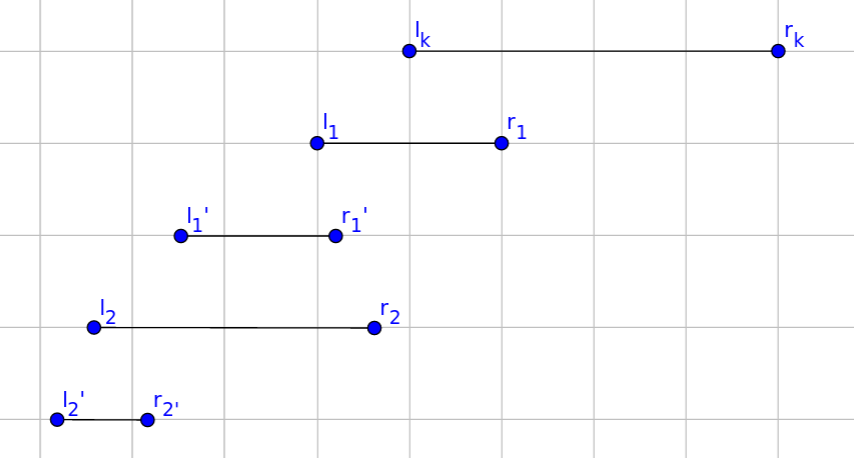
\includegraphics[scale=0.20]{case1.png}
        \caption{case 1.}
        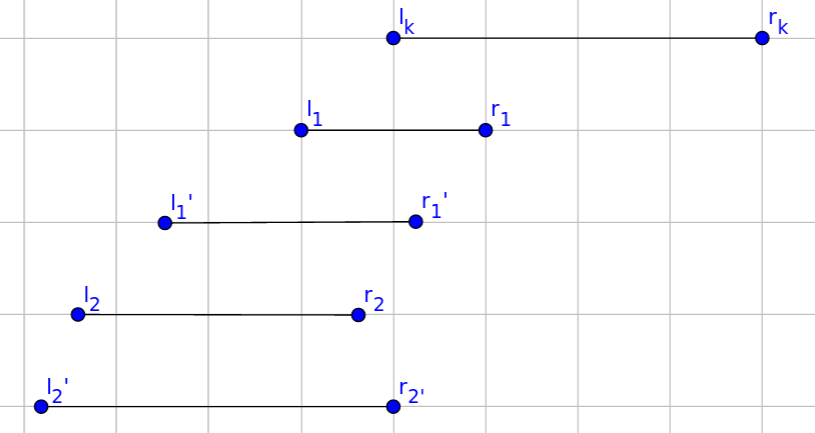
\includegraphics[scale=0.20]{case_2.png}
        \caption{case 2.}
    \end{figure}

    \textit{Induction step}\\
    The induction step is proved in exactly the same way, by replacing $i_k$ by $j_p'$; $j_1, j_1'$ by $j_{p+1}, j_{p+1}'$, etc.\\
    
    \textit{Conclusion}\\
    In definitive, we have $r_m' < r_1' < r_k$. It is thus a contradiction with the fact that $j_m' \cap i_n \ne \emptyset$.

\end{proof}

\end{document}